Database testing is performed in a dynamic white-box manner. The tests are white-box as it is not the MySQL server we are testing, but rathers that the database design
corresponds to the functionality which is expected. A total of 16 test cases have been designed, \autoref{fig:dbtest01-12} shows the test design for test cases \#0000 to \#0011.
The identifier \code{TD0001} points to the table in \autoref{fig:dbtd0001}, which explains each step to be performed for the test cases in \autoref{fig:dbtest01-12}.


\begin{figure}[H]
 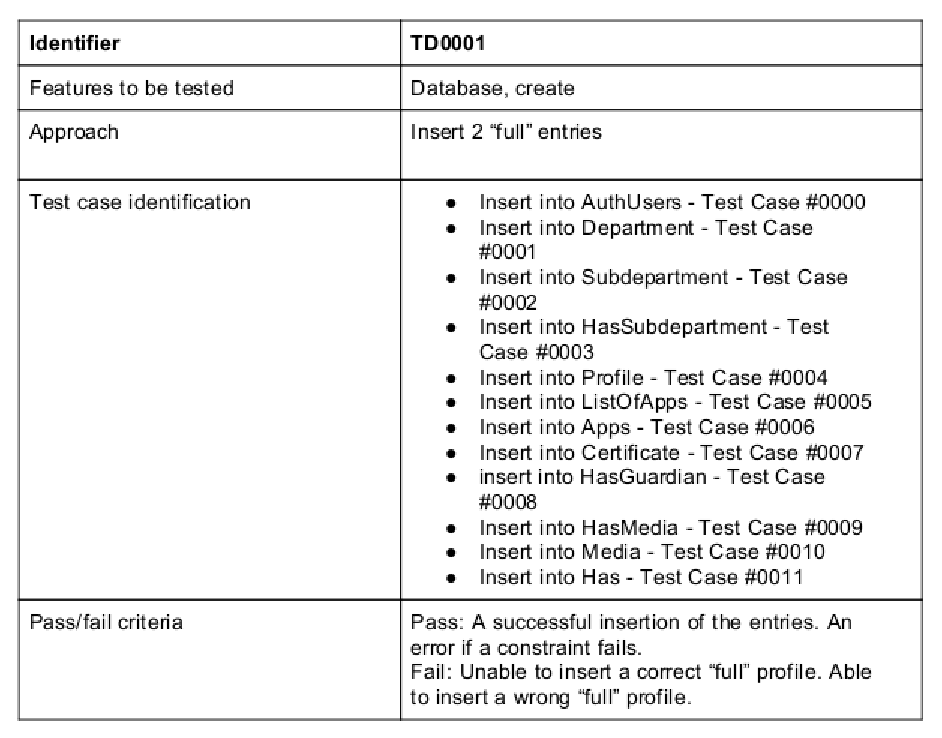
\includegraphics[scale=1.00]{images/dbtesttd0001}
 \caption{Testcase design of tests \#0000 to \#0011.}
  \label{fig:dbtest01-12}
\end{figure}

\begin{figure}[H]
 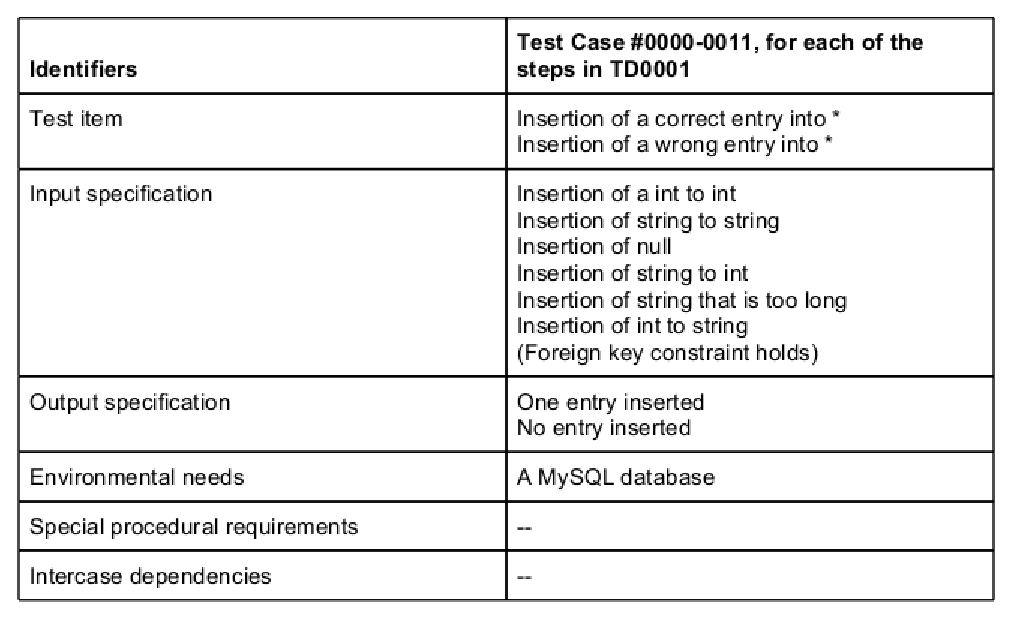
\includegraphics[scale=1.00]{images/dbtestcase01-12}
  \caption{Testcases \#0000 to \#0011}
  \label{fig:dbtd0001}
\end{figure}

All the database tests are done manually and require human interpretation. \autoref{hej} shows an example of the test output, in this particular case attempting
to insert a user-name longer than the allowed 45 characters. 


\begin{Code}
\begin{lstlisting}[label=hej,caption=Test case output]
--------------
INSERT INTO AuthUsers
values('tolongstring',null,1,
       'username00username00username00username00username00',
       'hansen')
--------------

ERROR 1406 (22001): Data too long for column 'username' at row 1
\end{lstlisting}
\end{Code}

Remaining test designs and cases can be found in \ref{app:dbTest}.